% PGF heart plot marks used at force-vector measurement points.
\documentclass[border=2pt]{standalone}
\usepackage{tikz}
\usetikzlibrary{arrows.meta,plotmarks}

\begin{document}
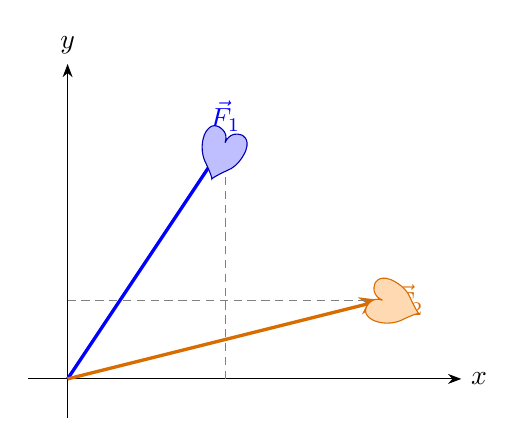
\begin{tikzpicture}[>=Stealth]
  \draw[->] (-0.5,0) -- (5,0) node[right] {$x$};
  \draw[->] (0,-0.5) -- (0,4) node[above] {$y$};
  \draw[very thick,blue,-Stealth] (0,0) -- (2,3)
    node[above] {$\vec F_1$};
  \draw[very thick,orange!85!black,-Stealth] (0,0) -- (4,1)
    node[right] {$\vec F_2$};
  \draw[densely dashed,gray] (2,0) -- (2,3);
  \draw[densely dashed,gray] (0,1) -- (4,1);
  \draw[blue!70!black,fill=blue!25,mark size=8pt]
    plot[mark=heart,mark options={rotate=-20}] coordinates {(2,3)};
  \draw[orange!85!black,fill=orange!30,mark size=8pt]
    plot[mark=heart,mark options={rotate=70}] coordinates {(4,1)};
\end{tikzpicture}
\end{document}
